\documentclass[12pt]{article}
\usepackage{amsmath}
\usepackage{times}
\usepackage{graphicx}
\usepackage{color}
\usepackage{multirow}
%
\usepackage[authoryear]{natbib}
%
\usepackage{rotating}
\usepackage{bbm}
\usepackage{latexsym}
%
\usepackage{tikz}
\usetikzlibrary{shapes.geometric, arrows}

%%% margins 
\textheight 23.4cm
\textwidth 14.65cm
\oddsidemargin 0.375in
\evensidemargin 0.375in
\topmargin  -0.55in
%
\renewcommand{\baselinestretch}{2}
%
\interfootnotelinepenalty=10000
%
\renewcommand{\thesubsubsection}{\arabic{section}.\arabic{subsubsection}}
\newcommand{\myparagraph}[1]{\ \\{\em #1}.\ \ }
\newcommand{\citealtt}[1]{\citeauthor{#1},\citeyear{#1}}
\newcommand{\myycite}[1]{\citep{#1}}

% Different font in captions
\newcommand{\captionfonts}{\normalsize}

\makeatletter  
\long\def\@makecaption#1#2{%
  \vskip\abovecaptionskip
  \sbox\@tempboxa{{\captionfonts #1: #2}}%
  \ifdim \wd\@tempboxa >\hsize
    {\captionfonts #1: #2\par}
  \else
    \hbox to\hsize{\hfil\box\@tempboxa\hfil}%
  \fi
  \vskip\belowcaptionskip}
\makeatother   
%%%%%

\renewcommand{\thefootnote}{\normalsize \arabic{footnote}} 	

\begin{document}
\hspace{13.9cm}1

\ \vspace{20mm}\\

{\LARGE Insert title here....}

\ \\
{\bf \large Pratik S. Sachdeva$^{\displaystyle 1, \displaystyle 2}$, Michael R. DeWeese$^{\displaystyle 1, \displaystyle 2}$}\\
{$^{\displaystyle 1}$Redwood Center for Theoretical Neuroscience.}\\
{$^{\displaystyle 2}$University of California, Berkeley.}\\
%

%\ \\[-2mm]
{\bf Keywords:} Neural variability, noise correlations, shared and private noise, synaptic weighting

\thispagestyle{empty}
\markboth{}{NC instructions}
%
\ \vspace{-0mm}\\
%
%Abstract
\begin{center} {\bf Abstract} \end{center}
This documentation briefly describes the formats required by Neural Computation. We hope this will help you with the manuscript preparation.
%%%%%%%%%%%

\section{Introduction}
Variability is a prominent feature of neural systems: neural responses to external stimuli will vary trial-to-trial even when the stimuli are constant. In particular, neural variability exhibits pairwise correlations: these ``noise correlations'' have been observed throughout the cortex. They have long been of theoretical interest because their presence has strong implications for neural coding.

From a population coding perspective, a neural population must produce a faithful representation of relevant quantities for their computation. One advantage of population coding is that variability unique to each neuron, or private variability, can be averaged out. If some variability is shared across neurons, i.e. we have noise correlations, larger populations of neurons cannot naively average out the variability. An abundance of theoretical work has explored how shared variability, therefore, can be both detrimental or beneficial to the fidelity of a population code depending on its structure. A  general conclusion of this theoretical work highlights the importance of the geometric relationship between the signal and noise correlations (both of which are stimulus-dependent).

Thus, the sources of neural variability - and their respective contributions to the private and shared components - will have a significant impact on shaping the geometry of the population's correlational structure, and therefore coding ability. For example, private sources of variability such as channel noise or stochastic synaptic vesicle release could be averaged out by large populations of neurons. But sources of variability shared across neurons - such as the variability of presynaptic spike trains - would induce noise correlations and place different constraints on our neural code.  Indeed, any variability carried by an incoming stimulus possesses would also introduce variability in the population. Such ``shared input noise'' is particularly detrimental to the fidelity of a population code \cite{Moreno-Bote2014, Kanitscheider2015}.

In prior work, we examined the private and shared variability in the auditory cortex. Specifically, we partitioned sub-threshold variability into private components (synaptic, thermal, and other local sources of variability) and shared components (variability induced by afferent connections). We found that the private component of the total variability is quite small, while the shared component can be much larger (Figure \ref{fig:private-shared}B). Thus, the large shared component of a neuron's variability, a source of noise correlations, has important consequences for neural coding.

We sought out to explore how shared and private sources of neural variability interact to influence neural coding. As mentioned before, work by Moreno-Bote et al. demonstrated that shared input noise is detrimental to the fidelity of a population code. Here, we instead turn to sources of shared variability which are not carried by stimulus and thus can be manipulated by features of neural computation such as synaptic weighting. We refer to these noise sources as ``common noise'' to distinguish them from the special case of ``shared input noise.'' For example, a common noise source could include an upstream neuron whose action potentials are ``noisy'' in the sense that they are unimportant for the computation of the current stimulus.

Thus, we explored how common private noise impact neural coding. We consider a very simple linear-nonlinear architecture and  

\section{Methods}

\subsection{Network Architecture}
We consider the linear-nonlinear architecture depicted in Figure \ref{architecture}. The inputs to the network consist of a stimulus $s$ along with common (Gaussian) noise $\xi_C$. The $N$ neurons in the network take a linear combination of the inputs which is then corrupted by i.i.d. private Gaussian noise. Thus, the output of the linear stage for the $i$th neuron is 
\begin{align}
\ell_i &= v_i s + w_i \sigma_C \xi_C + \sigma_P\xi_{P,i},
\end{align}
where $\xi_{P,i}$ is the private noise. Both noise terms are scaled by positive constants $\sigma_C$ and $\sigma_P$ in order to make their variances explicit. The noisy linear combination is passed through a nonlinearity $g_i(\ell_i)$ whose output $r_i$ can be thought of as a firing rate. We consider the cases in which $\mathbf{r}$ alone serves as the network's output and when it acts as the mean for a Poisson firing process.

Thus, the network-wide computation is given by
\begin{align}
\mathbf{r} &= \mathbf{g}(\mathbf{v} s + \mathbf{w} \sigma_C \xi_C +\sigma_P \boldsymbol{\xi}_P)
\end{align}
where vector notation denotes the weights, noises, and nonlinearities across the neuronal population. In this scheme the correlational structure of the network is dictated by the choice of weight vectors $\mathbf{v}$, $\mathbf{w}$ along with the array of nonlinearities $\mathbf{g}$. 
\begin{figure}[ht]
	\centering
	\scalebox{1.0}{
		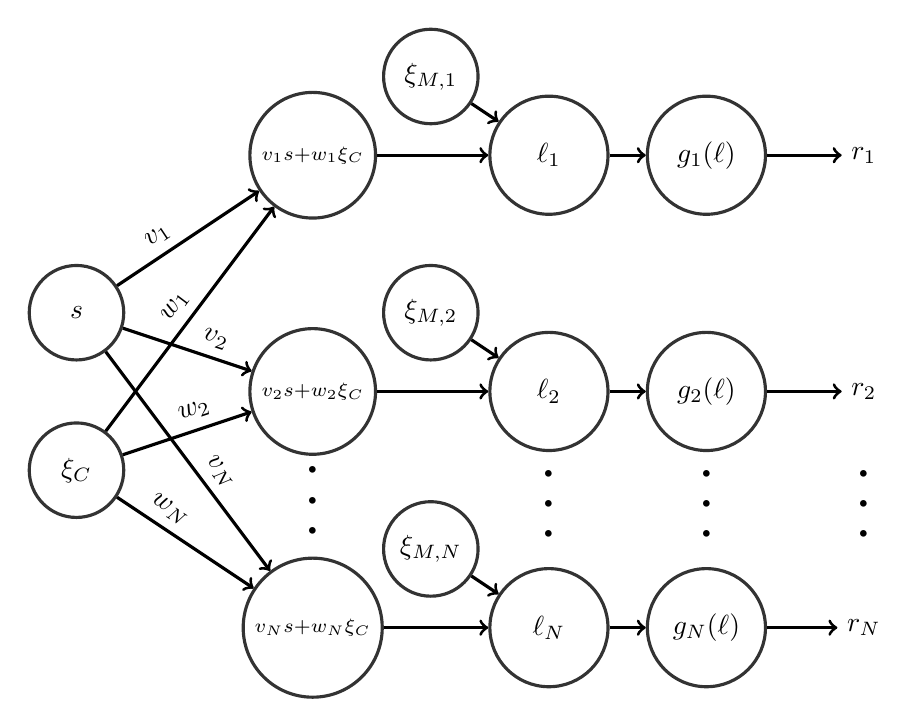
\begin{tikzpicture}
		\tikzstyle{main} = [circle, minimum size = 12mm, line width = 0.4mm, draw=black!80, node distance = 16mm]
		\tikzstyle{main2} = [circle, minimum size = 15mm, line width = 0.4mm, draw=black!80, node distance = 16mm]
		\node[main, fill = white!100] at (-2, 1.) (s) {$s$};
		\node[main, fill = white!100] at (-2, -1.) (common) {$\xi_C$};
		
		\node[main2] at (1.,3.0)  (l1) {${\scriptstyle v_1 s + w_1 \xi_C}$};
		\node[main2] at (1.,0.0)  (l2) {${\scriptstyle v_2 s + w_2 \xi_C}$};
		\node[main2] at (1,-3.0) (lN) {${\scriptstyle v_N s + w_N \xi_C}$};
		
		\node[main2] at (4.,3.0)  (ell1) {$\ell_1$};
		\node[main2] at (4.,0.0)  (ell2) {$\ell_2$};
		\node[main2] at (4,-3.0) (ellN) {$\ell_{N}$};
		
		\node[main2] at (6, 3.0) (nonlin1) {$g_1(\ell)$};
		\node[main2] at (6, 0.0) (nonlin2) {$g_2(\ell)$};
		\node[main2] at (6, -3.0) (nonlinN) {$g_N(\ell)$};
		
		\node at (8, 3.0) (r1) {$r_1$};
		\node at (8, 0.0) (r2) {$r_2$};
		\node at (8, -3.0) (rN) {$r_N$};
		
		\node[main] at (2.5, 4.0) (xi1) {$\xi_{M,1}$};
		\node[main] at (2.5, 1.0) (xi2) {$\xi_{M,2}$};
		\node[main] at (2.5, -2.0) (xiN) {$\xi_{M,N}$};
		
		\draw[->, line width = 0.4mm] (s) -- (l1) node[midway, above left, sloped] {$v_1$};
		\draw[->, line width = 0.4mm] (s) -- (l2) node[midway, above right, sloped] {$v_2$};
		\draw[->, line width = 0.4mm] (s) -- (lN) node[midway, above right, sloped] {$v_N$};
		
		\draw[->, line width = 0.4mm] (common) -- (l1) node[pos = 0.6, above left, sloped] {$w_1$};
		\draw[->, line width = 0.4mm] (common) -- (l2) node[pos = 0.8, above left, sloped] {$w_2$};
		\draw[->, line width = 0.4mm] (common) -- (lN) node[midway, above left, sloped] {$w_N$};
		
		\draw[->, line width = 0.4mm] (l1) -- (ell1);
		\draw[->, line width = 0.4mm] (l2) -- (ell2);
		\draw[->, line width = 0.4mm] (lN) -- (ellN);
		
		\draw[->, line width = 0.4mm] (xi1) -- (ell1);
		\draw[->, line width = 0.4mm] (xi2) -- (ell2);
		\draw[->, line width = 0.4mm] (xiN) -- (ellN);
		
		\draw[->, line width = 0.4mm] (ell1) -- (nonlin1);
		\draw[->, line width = 0.4mm] (ell2) -- (nonlin2);
		\draw[->, line width = 0.4mm] (ellN) -- (nonlinN);
		
		\draw[->, line width = 0.4mm] (nonlin1) -- (r1);
		\draw[->, line width = 0.4mm] (nonlin2) -- (r2);
		\draw[->, line width = 0.4mm] (nonlinN) -- (rN);
		
		\path (l2) -- (lN) node [black, font=\Huge, midway, sloped] {$\dots$};
		\path (ell2) -- (ellN) node [black, font=\Huge, midway, sloped] {$\dots$};
		\path (nonlin2) -- (nonlinN) node [black, font=\Huge, midway, sloped] {$\dots$};
		\path (r2) -- (rN) node [black, font=\Huge, midway, sloped] {$\dots$};	
		\end{tikzpicture}}
	
	\caption{Linear-Nonlinear Network Architecture. The network takes as its inputs a stimulus $s$ and common noise $\xi_C$. A linear combination of these quantities is corrupted by individual membrane potential noise $\xi_{P,i}$. The output of this linear stage is then passed through a nonlinearity $g_i(\ell)$.}
	\label{architecture}
\end{figure}

\subsection{Measures of Coding Strength}
In order to assess the fidelity of the population code represented by $\boldsymbol{\ell}$ or $\mathbf{r}$, we turn to the Fisher information and the Shannon mutual information. The former has largely been utilized in the context of sensory decoding and correlated variability \cite{2016kohn} while the latter has been well studied in the context of efficient coding. 

The Fisher information sets a limit by which the readout of a population code can determine the value of the stimulus. Formally, it sets a lower bound to the variance of an unbiased estimator for the stimulus. Often, the Fisher information is intractable to calculate analytically; a suitable lower bound is the linear Fisher information:
\begin{align}
I_F(s) &= \mathbf{f}'(s)^T \boldsymbol{\Sigma}^{-1}(s) \mathbf{f}(s)
\end{align}
whose corresponding estimator is the locally optimal linear estimator. 

The Shannon mutual information quantifies the reduction in uncertainty of one random variable given knowledge of another. In the context of Figure \ref{architecture}, we are interested in the mutual information between the neural representation $\mathbf{r}$ and the stimulus $s$, i.e. $I[s, \mathbf{r}]$. As with the Fisher information, the mutual information is often not analytically tractable. Thus, we turn to the abundance of work devoted to formulating estimators of the mutual information from data. Specifically, we will utilize the nearest-neighbor estimator developed by Kraskov et al. 
\subsection{Structured Weights}
To obtain analytic expressions for these quantities, we first consider the case of ``structured weights'' taking on the form
\begin{align}
c \times \left(\underbrace{1 \cdots 1}_{N/k \text{ times}}  \ \underbrace{2 \cdots 2}_{N/k \text{ times}} \ \cdots \ \underbrace{k \cdots k}_{N/k \text{ times}}   \right)^T.
\end{align}
Specifically, the structured weight vectors are parameterized by an integer $k$ which divides the $N$ weights into $k$ homogeneous groups. The weights across the groups span the positive integers up to $k$, and we allow for a final scaling factor $c$. 

Importantly,  larger $k$ will only increase the weights in the vector. Thus, in the above scheme, increased ``diversity'' can only be achieved through an increase through the parameter $k$, which will invariably result in an amplification of the signal to which the weight vector is applied. In the case that $k$ does not evenly divide $N$, the last group is repeated $N\text{mod }k$ times.

Lastly, we will consider cases when $k$ is of the order $N$, e.g. $k = N/2$. Such a value of $k$ ensures that the weights grow with the population size. This is in contrast for $k$ a constant, such as $k=4$, which sets a maximum weight size no matter the population size. 
\subsection{Unstructured Weights}

While the structured weights provide us analytic results, they possess an unrealistic distribution of synaptic weighting. Thus, we turn to the case of ``unstructured weights,'' in which the synaptic weights are drawn from some parameterized probability distribution:
\begin{align}
\mathbf{v} \sim p(\mathbf{v}; \theta_{\mathbf{v}}); \ \mathbf{w} \sim p(\mathbf{w}; \theta_{\mathbf{w}}).
\end{align}
Thus, we  calculate both information theoretic quantities over many random draws from these distributions. We then observe how the quantities behave as some subset of the parameters $\theta$ are varied. In particular, we will focus on the lognormal distribution, which has been observed to describe the distribution of synaptic weights well in slice electrophysiology \textcolor{red}{[citation]}. Specifically, we examine 
\begin{align}
\mathbf{w}\sim \text{Lognormal}(\mu - \Delta, \sigma)
\end{align}
where $\Delta$ sets a lower bound for the weights. Here, increased ``diversity'' in the sense of the structured weights is achieved by increasing $\mu$, which increases the mean, median, and mode of the lognormal distribution. This is in contrast with increasing $\sigma$, which will decrease the mode of the distribution.

\section{Citations}
The citations must follow the APA format. A typical citation is given by $\backslash citep$, for example \citep{Ref2009}. The command $\backslash cite$ will generate \cite{Ref2009}. For references with multiple authors, the command $\backslash citet$ will generate \citet{Ref2008} and $\backslash citep$ will generate \citep{Ref2008}. To put texts in the reference, use command $\backslash citep[see, e.g.,][for instance]\{Ref2009\}$ which generates \citep[see,
e.g.,][for instance]{Ref2009}. To cite multiple references, use the command $\backslash citep\{ref1,ref2,ref3\}$, for example \citep[compare][]{Ref2008,Ref2009}.

For Neural Computation, the $\backslash citep$ is preferred.




\section*{Conclusion}
We have illustrated the basic format to the manuscript that you consider to submit to Neural Computation. We hope this is helpful to the authors.

\subsection*{Acknowledgments}


\section*{Appendix}
You should put the details that are not required in the main body into this Appendix.

\begin{thebibliography}{100}
\providecommand{\natexlab}[1]{#1}
\expandafter\ifx\csname urlstyle\endcsname\relax
  \providecommand{\doi}[1]{doi:\discretionary{}{}{}#1}\else
  \providecommand{\doi}{doi:\discretionary{}{}{}\begingroup
  \urlstyle{rm}\Url}\fi

\bibitem[{LastName(2009)}]{Ref2009}
LastName, A. (2009).
\newblock Title for the first reference.
\newblock \emph{Journal of the first reference}, \emph{3}, 18 -- 88.


\bibitem[{Authors et~al.(2008)Author1, Author2, \&
  Author3}]{Ref2008}
Author1, A., Author2, A., \& Author3, A. (2008).
\newblock Title for the second reference.
\newblock \emph{Journal for the second reference}, \emph{5}, 188 -- 200.

\end{thebibliography}
\end{document}